\noindent

\includegraphics[height=1.25cm]{images/pictograms/benchmark}

\includegraphics[height=1.25cm]{images/pictograms/FEM}
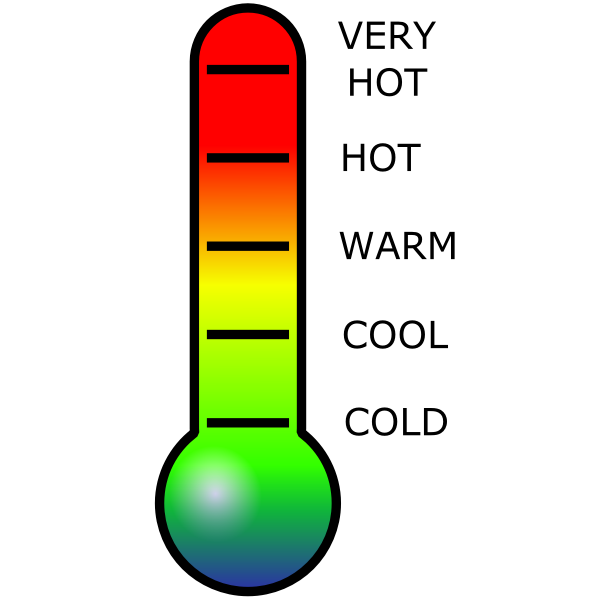
\includegraphics[height=1.25cm]{images/pictograms/temperature}

\includegraphics[height=1.25cm]{images/pictograms/3d}

\includegraphics[height=1.25cm]{images/pictograms/paraview}

%%%%%%%%%%%%%%%%%%%%%%%%%%%%%%%%%%%%%%%%%%%%%%%%%%%%%%%%%%%%%%%%%%%%%%%%%%%%%%%%%%%%%%%%%%%%%%%%%%%

\begin{flushright} {\tiny {\color{gray} python\_codes/fieldstone\_177/text.tex}} \end{flushright}

\par\noindent\rule{\textwidth}{0.4pt}

\begin{center}
\inpython
{\small Code: \url{https://github.com/cedrict/fieldstone/tree/master/python_codes/fieldstone_177}}
\end{center}

\par\noindent\rule{\textwidth}{0.4pt}

Last revision: September 13th, 2025.

\par\noindent\rule{\textwidth}{0.4pt}

%%%%%%%%%%%%%%%%%%%%%%%%%%%%%%%%%%%%%%%%%%%%%%%%%%%%%%%%%%%%%%%%%%%%%%%%%%%%%%%%%%%%%%%%%%%%%%%%%%%

This \stone presents a more compact way of building the energy equation FE matrix. 
The basic equation we solve here is
\[
\rho C_p \left( \frac{\partial T}{\partial t} + \vec\upnu \cdot \vec\nabla T \right)
= \vec\nabla \cdot k \vec\nabla T 
\]
In what follows we use trilinear $(Q_1)$ elements.
The FEM discretization of the energy equation is presented in Chapter~\ref{MMM-chapt5}.
In what follows I will omit the standard parts of the code as well as the time loop, export to vtu, etc ...
to focus on the 'new' aspects.

%==================================
\section*{Implementation}

Note that the 'new' method requires to have the connectivity 
array transposed with regards to how I normally define it.

We start with creating three arrays which contain 
the local coordinates of the element nodes:
\begin{lstlisting}
r_T=np.array([-1, 1, 1,-1,-1, 1, 1,-1],np.float64)
s_T=np.array([-1,-1, 1, 1,-1,-1, 1, 1],np.float64)
t_T=np.array([-1,-1,-1,-1, 1, 1, 1, 1],np.float64)
\end{lstlisting}

Then a list of quadrature point coordinates and weights is created
(the first 3 values are the $r,s,t$ coordinates, the 4th one is the weight):
\begin{lstlisting}
a=1/np.sqrt(3)
quadrature_points = [(-a,-a,-a ,1),
                     ( a,-a,-a ,1) , 
                     ( a, a,-a ,1) ,
                     (-a, a,-a ,1) ,
                     (-a,-a, a ,1) , 
                     ( a,-a, a ,1) , 
\end{lstlisting}

The FE matrix is defined as a row-based LIst of Lists sparse 
matrix\footnote{\url{https://docs.scipy.org/doc/scipy/reference/generated/scipy.sparse.lil_matrix.html}}:
\begin{lstlisting}
    A_fem=lil_matrix((Nfem,Nfem),dtype=np.float64)
\end{lstlisting}

For simplicity, and since all elements are identical cuboids of size $(h_x,h_y,h_z)$
the Jacobian determinant and the Jacobian inverse are computed simply as
\begin{lstlisting}
jcbi=np.diag([2/hx,2/hy,2/hz])
jcob=hx*hy*hz/8
\end{lstlisting}

We then of course proceed to loop over elements, 
by means of the \lstinline{enumerate} 
function\footnote{\url{https://www.w3schools.com/python/ref_func_enumerate.asp}}
and retrieve the node velocity and temperature:

\begin{lstlisting}
    for e,nodes in enumerate(icon_T):
        ue,ve,we,Te=u[nodes],v[nodes],w[nodes],Told[nodes]
\end{lstlisting}

We then loop over the quadrature points, again with the \lstinline{enumerate}
function:
\begin{lstlisting}
        for rq,sq,tq,weightq in quadrature_points:
\end{lstlisting}
Since \lstinline{rnodes,snodes, tnodes} are arrays we can 
elegantly compute the basis functions and their derivatives as follows
(the arrays have shape \lstinline{(8,)}):
\begin{lstlisting}
            N_T=0.125*(1+r_T*rq)*(1+s_T*sq)*(1+t_T*tq)
            dNdr_T=0.125*r_T*(1+s_T*sq)*(1+t_T*tq)
            dNds_T=0.125*s_T*(1+r_T*rq)*(1+t_T*tq)
            dNdt_T=0.125*t_T*(1+r_T*rq)*(1+s_T*sq)
\end{lstlisting}

Instead of building \lstinline{dNdx,dNdy,dNdz} we directly build the 
${\bm B}$ gradient matrix as follows (which has shape \lstinline{(8,3)}:
\begin{lstlisting}
            B=(jcbi@np.vstack((dNdr_T,dNds_T,dNdt_T))).T
\end{lstlisting}
The elemental mass and diffusion matrices are then very straightforwardly built
(note that \lstinline{A@B} is equivalent to \lstinline{dot(A,B)}:
\begin{lstlisting}
            MM+=rho*hcapa*np.outer(N_T,N_T)*jcob*weightq
            Kd+=B@B.T*hcond*jcob*weightq
\end{lstlisting}
Concerning the advection matrix we first build the 
velocity vector at the quadrature point using the 
basis functions (\lstinline{velq} has shape \lstinline{(3,)} shape),
then precompute $\vec\upnu \cdot {\bm B}$ of \lstinline{(8,)} shape,
and finally the matrix using \lstinline{outer} (note that 
one should check Ka is indeed correct here).

\begin{lstlisting}
            velq=np.dot(N_T,np.vstack((ue,ve,we)).T)
            advN=B@velq # (8,) shape
            Ka+=np.outer(N_T,advN)*jcob*weightq*rho*hcapa
\end{lstlisting}

Once the loop over quadrature points completed
we can compute the elemental matrix and rhs where
$\alpha=1/2$ yields a Crank-Nicolson scheme: 
\begin{lstlisting}
        A_el=MM+alphaT*(Ka+Kd)*dt
        b_el=(MM-(1-alphaT)*(Ka+Kd)*dt).dot(Te)
\end{lstlisting}

Boundary conditions are imposed on the elemental matrix and rhs, as standard.
Finally the assembly is carried out in an elegant manner, using the \lstinline{ix_}
function:

\begin{lstlisting}
        A_fem[np.ix_(nodes,nodes)]+=A_el
        b_fem[nodes]+=b_el
\end{lstlisting}

For comparison, I have also implemented the 'old' way of building the 
matrix that we find in \stone~20. That approach could of course be 
easily improved on, but I leave 'as is' and use it as an end member.

%==================================
\section*{Experiments}

Experiment 1 is a simple diffusion problem.

Experiment 2 is an advection-diffusion problem with the velocity field given by 
\begin{lstlisting}
   u[:] = x_T*(1-x_T)*(1-2*y_T)*(1-2*z_T)    *10
   v[:] = (1-2*x_T)*y_T*(1-y_T)*(1-2*z_T)    *10
   w[:] = -2*(1-2*x_T)*(1-2*y_T)*z_T*(1-z_T) *10
\end{lstlisting}

%==================================
\section*{Results}

Various timings are measured for both old and new approach 
of building the FE matrix as a function of number of dofs (resolutions 
from $8^3$ to $24^3$ elements):

\begin{center}
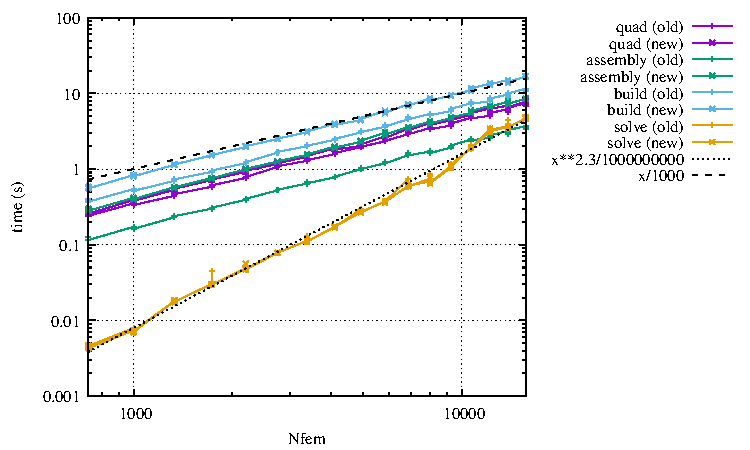
\includegraphics[width=15cm]{python_codes/fieldstone_177/RESULTS/times.pdf}
\end{center}

we find that:
\begin{itemize}
\item quadrature loop to compute the elemental matrices take about the same time (purple lines) 
\item assembly time is smaller for old than new (about 2.5 faster)!!
\item total global FEM matrix building time is linear but old is about 20-25\% faster !
\end{itemize}


\includegraphics[width=3cm]{images/conclusion}
This 'new' method is somewhat elegant, may be more python-like, 
but slower than my initial naive take of \stone~20. 



